\chapter{Konzeption}
In diesem Kapitel wird der konzeptionelle Entwurf der entwickelten Lösung detailliert beschrieben. Die Konzeption umfasst alle wesentlichen Aspekte der Benutzeroberfläche, der Prozessabläufe sowie der Systemarchitektur. Dabei war es entscheidend, sowohl die technischen Anforderungen als auch die Nutzerbedürfnisse optimal zu berücksichtigen.
\newline
Zunächst werden die Mockups vorgestellt, die die geplanten Benutzeroberflächen visualisieren. Diese grafischen Entwürfe dienen als Grundlage für die spätere Implementierung der Benutzeroberfläche und helfen dabei, die Nutzerinteraktionen und das Design bereits in der frühen Phase des Projekts zu planen.
\newline
Daraufhin wird der Workflow des Anfrageprozesses dargestellt, um die Abfolge und Logik der einzelnen Prozessschritte zu veranschaulichen. Dies bildet die Grundlage für die spätere Implementierung der Abläufe und dient dazu, alle Beteiligten über die genauen Prozessschritte zu informieren.
\newline
Abschließend wird die Systemarchitektur präsentiert, die das fundamentale Gerüst der gesamten Anwendung bildet. Die Architektur beschreibt die wichtigsten Komponenten und deren Interaktionen, um eine stabile, skalierbare und erweiterbare Lösung zu gewährleisten.
\newpage
\section{Mockups}
Im Verlauf der Entwicklung des IAV Merida Request wurden regelmäßig Gespräche mit verschiedenen Stakeholdern geführt. Diese Interaktionen führten zur schrittweisen Anpassung der Mockups, die auf den gewonnenen Erkenntnissen basierten. Dadurch konnten die Mockups kontinuierlich an die sich entwickelnden Anforderungen und das gewünschte User Interface angepasst werden. Im Folgenden wird der Entwicklungsprozess der Mockups sowie deren verschiedene Versionen detailliert dargestellt.
\subsection*{Mockup 1}
In der ersten Version der Mockups, s. Abbildung \ref{fig:MockUps1.0}, orientierten sich die Designentscheidungen stark am BMW Request Channel. Die Struktur und die Benutzeroberfläche in dieser Phase waren relativ einfach gehalten, mit einem klaren Fokus auf die wesentlichen Eingabefelder und -optionen, die für das Anfordern von Daten und Analysen benötigt wurden.
\newline
Wichtige Merkmale dieser Version:
\begin{itemize}
    \item Eine klare und strukturierte Eingabe für persönliche Details, Datenanforderungen und den gewünschten Ausgabetyp (z.B. „Raw Data“ oder „Analysis“).
    \item Es wurde darauf geachtet, dass die Navigation zwischen den Schritten unkompliziert und intuitiv ist, allerdings war das Design noch stark an dem Layout des BMW Request Channel angelehnt.
\end{itemize}
\begin{figure}[H]
    \centering
    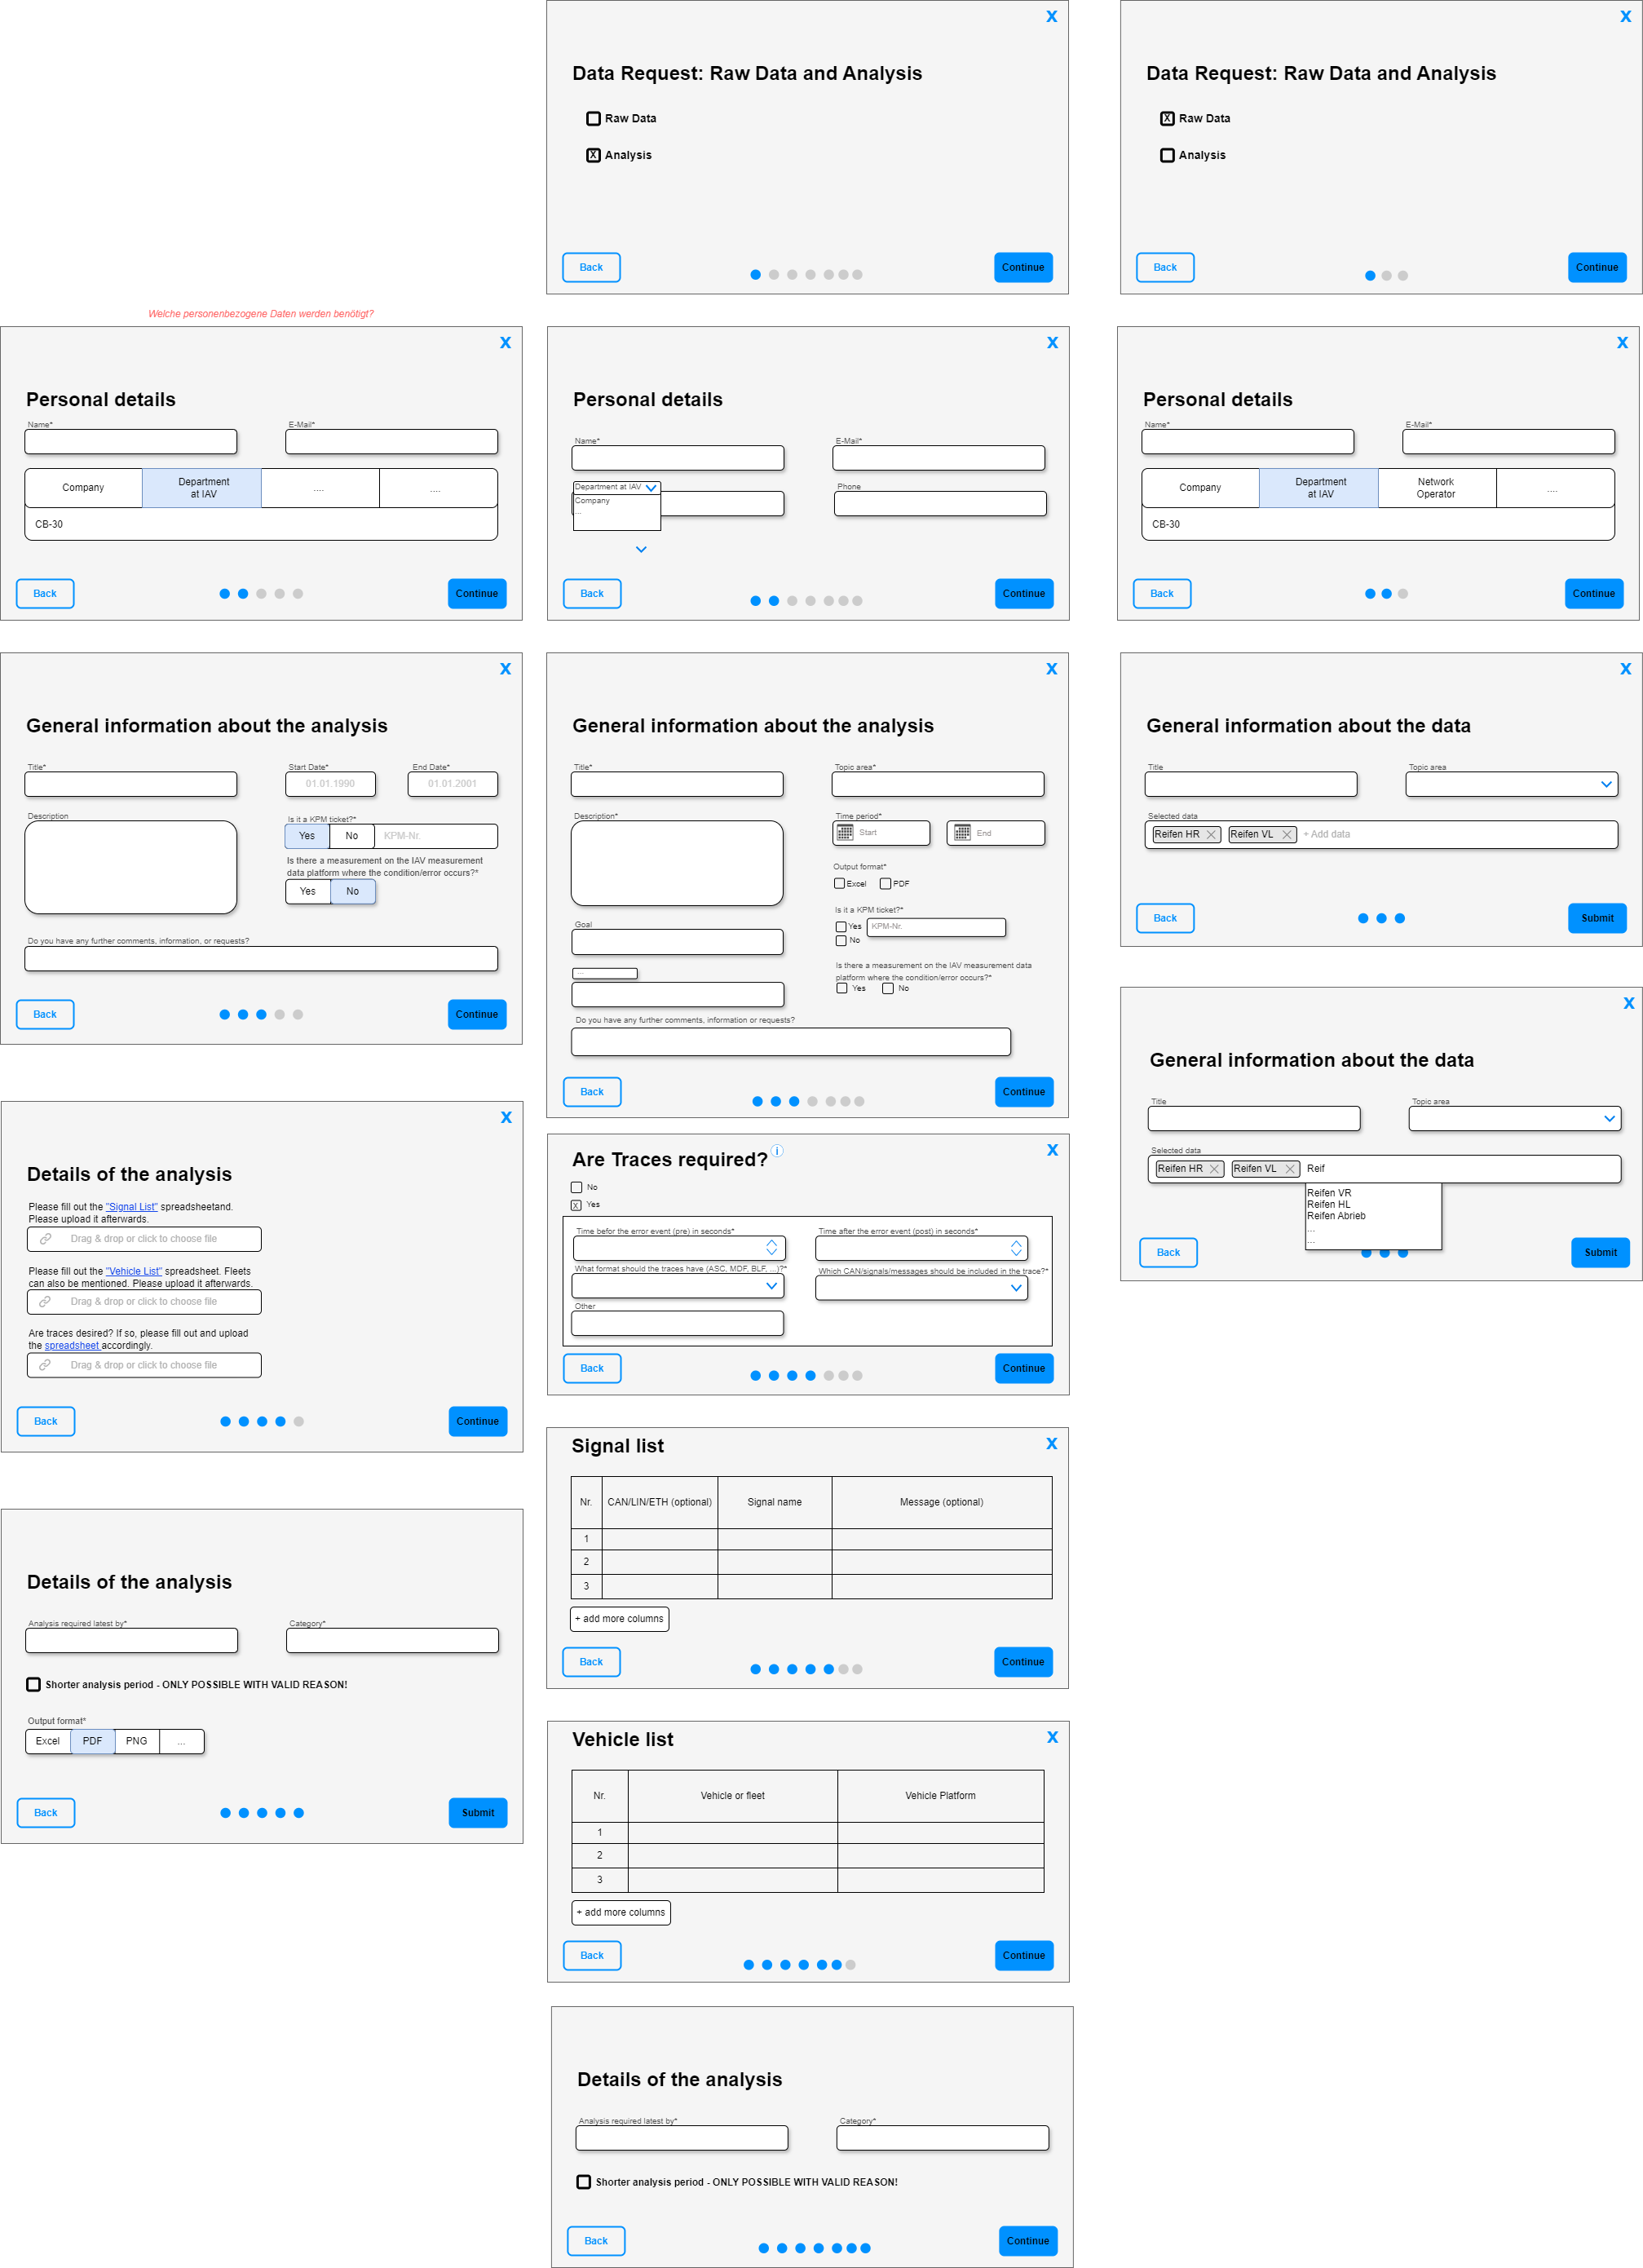
\includegraphics[scale=.2]{media/MockUps1.0}
    \caption{Mockup 1}
    \label{fig:MockUps1.0}
\end{figure}
\subsection*{Mockup 2}
Mit der zweiten Version, s. Abbildung \ref{fig:MockUps2.0}, wurde das Interface weiterentwickelt und dabei von der ursprünglichen BMW-Anlehnung gelöst. Es entstand ein individuelleres Design, das besser auf die spezifischen Anforderungen des Projekts zugeschnitten war. Dabei lag der Fokus auf einer verbesserten Benutzerführung und einer klareren Strukturierung der Formulare. Die Eingabefelder wurden optimiert, um eine bessere Lesbarkeit zu gewährleisten, und die Navigation wurde an den Workflow der Benutzer angepasst. Zusätzliche Hilfetexte und visuelle Hinweise führten den Benutzer durch den gesamten Anforderungsprozess. Diese Version stellte einen ersten großen Schritt in Richtung eines eigenständigen Tools dar.
\begin{figure}[H]
    \centering
    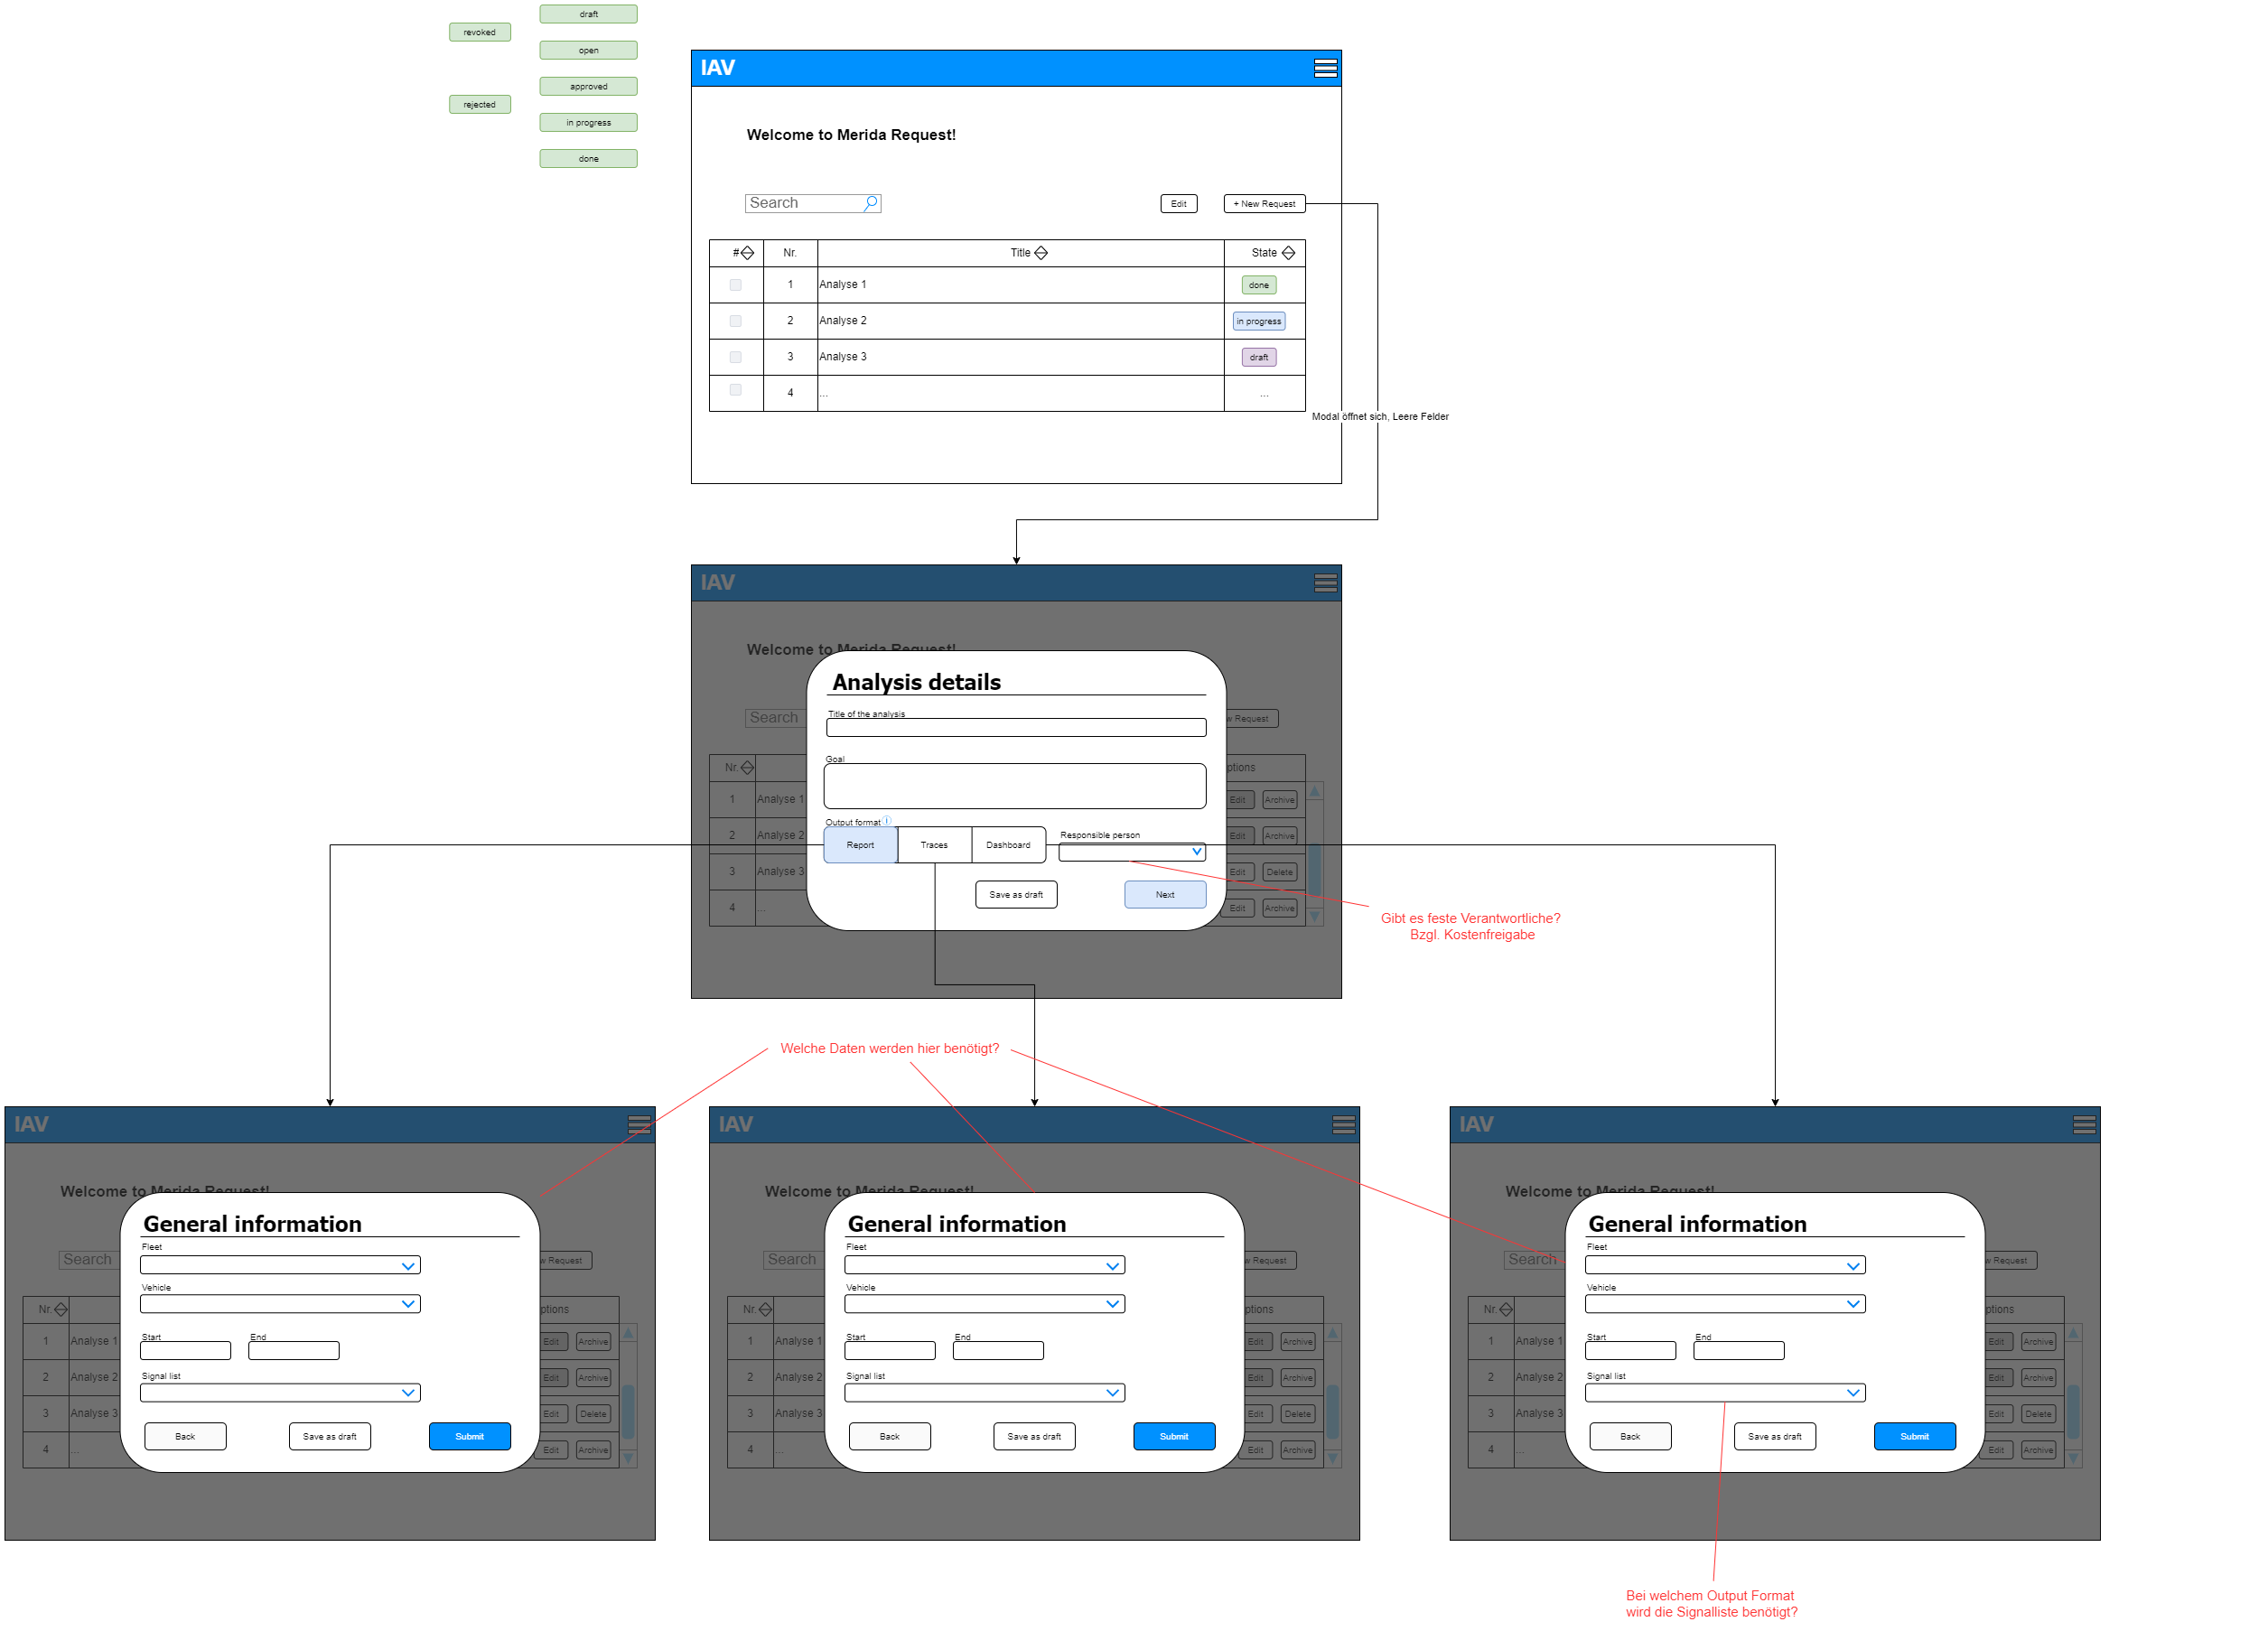
\includegraphics[scale=.2]{media/MockUps2.0}
    \caption{Mockup 2}
    \label{fig:MockUps2.0}
\end{figure}
\subsection*{Mockup 3 (Aktueller Stand)}
Das in der Abbildung \ref{fig:MockUps3.0} dargestellte Mockup repräsentiert den aktuellen Stand der Entwicklung und zeigt eine weiterentwickelte und verfeinerte Benutzeroberfläche. Hier liegt der Schwerpunkt auf dem Outputformat eines Dashboards und darauf, ein ausgereiftes und benutzerfreundliches System anzubieten, das sowohl funktional als auch optisch ansprechend ist.
\newline
Wichtige Änderungen in dieser Version:
\begin{itemize}
    \item Das Interface wirkt nun deutlich moderner und aufgeräumter. Es gibt eine klare Hierarchie in der Darstellung der Informationen, und die wichtigsten Optionen (wie die Auswahl des gewünschten Ausgabetyps) sind hervorgehoben.
    \item Die Benutzerführung wurde durch weitere Schritte verfeinert. Dazu gehören neue Kategorien für Diagrammtypen sowie eine präzisere Auswahloption für Flotten und Fahrzeuge. Die Auswahl erfolgt nun über eine Drag-and-Drop-Funktion, was die Bedienung vereinfacht und intuitiver gestaltet.
    \item Der Nutzer kann nun mehrere Diagramme im Stil eines Dashboards anlegen und konfigurieren. Am Ende des Prozesses erhält er eine zusammenfassende Übersicht über die erstellte Anfrage.
    \item Benutzer haben jetzt die Möglichkeit, Anfragen als Entwurf zu speichern und später weiterzubearbeiten. Diese Funktion erhöht die Effizienz und unterstützt eine flexible Arbeitsweise. 
\end{itemize}
\begin{figure}[H]
    \centering
    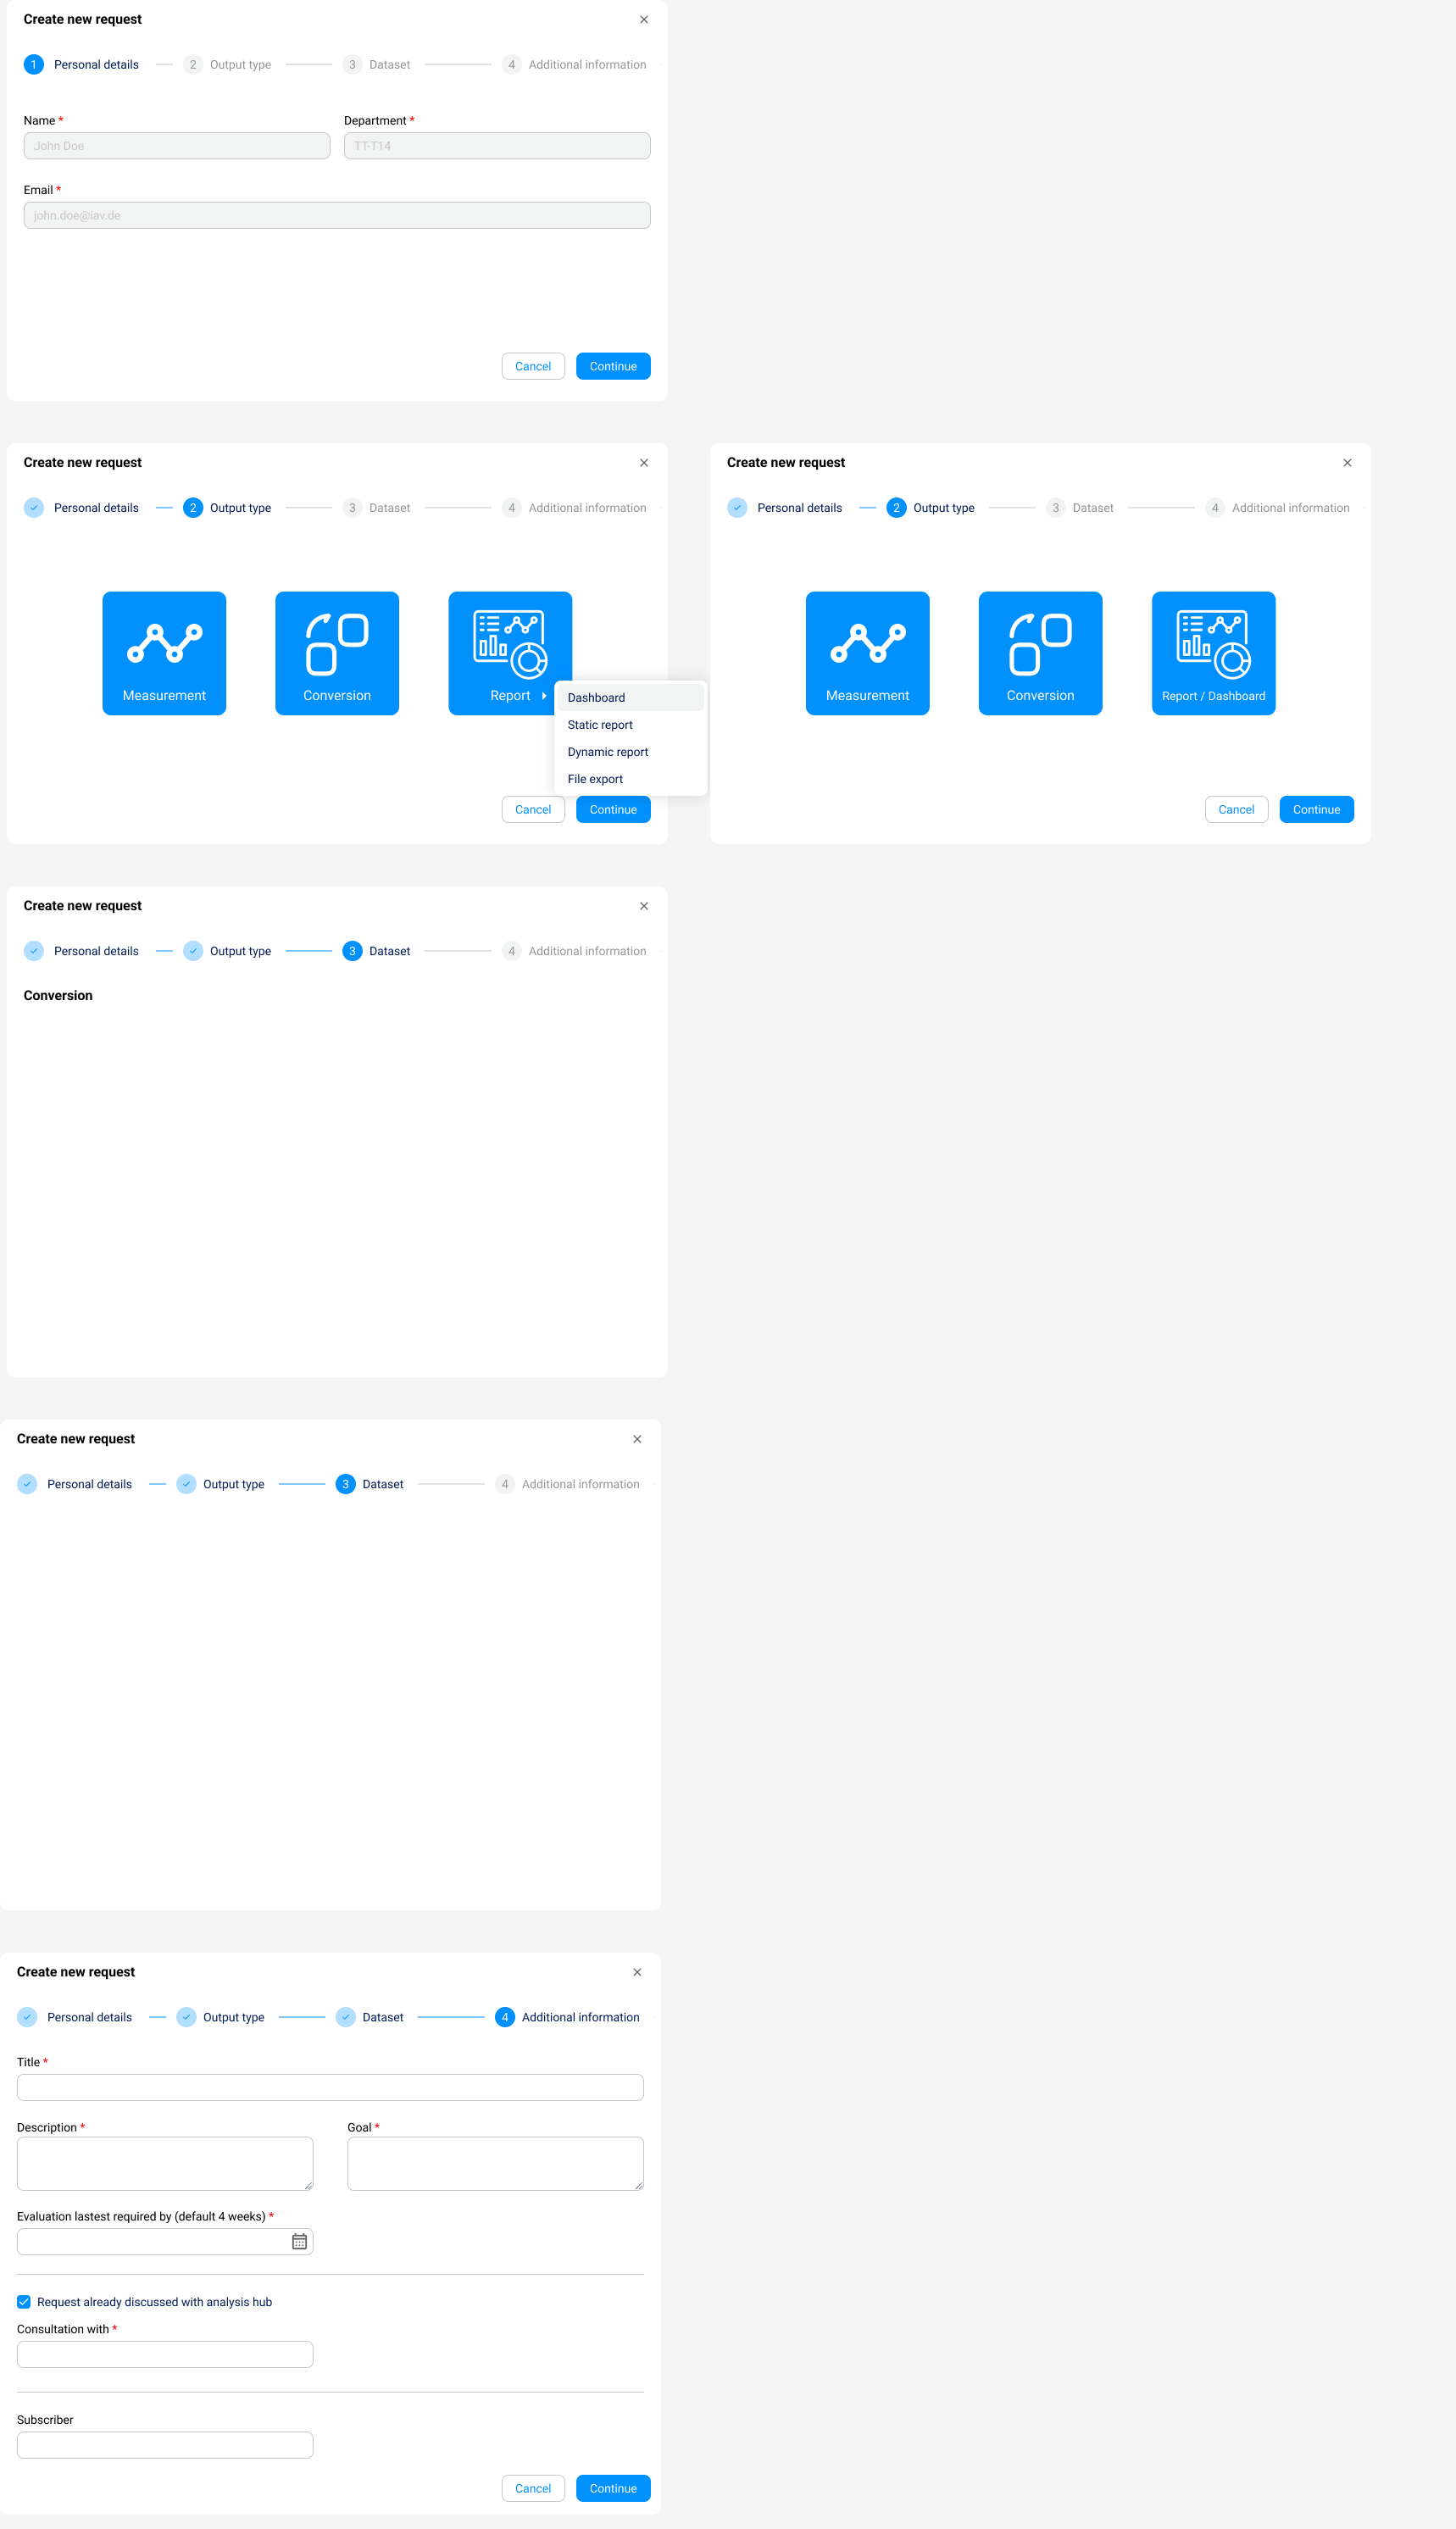
\includegraphics[scale=.25]{media/MockUps3.0}
    \caption{Mockup 3}
    \label{fig:MockUps3.0}
\end{figure}
Zusammenfassend lässt sich sagen, dass sich das IAV Merida Request Tool durch einen iterativen Entwicklungsprozess erheblich weiterentwickelt hat. Während Mockup 1 noch stark an bestehende Lösungen angelehnt war, strebte Mockup 2 bereits ein eigenständiges Design mit klareren Nutzerführungen an. Mit Mockup 3 erreicht das Tool nun ein hohes Maß an Benutzerfreundlichkeit, Flexibilität und Funktionalität, dass den Anforderungen der Benutzer in vollem Umfang gerecht wird.
\newpage
\section{Workflow}
Der dargestellte Workflow (s. Abbildung \ref{fig:Workflow}) beschreibt den vollständigen Ablauf eines Anfrageprozesses, der mehrere Phasen durchläuft, um eine effiziente und strukturierte Bearbeitung sicherzustellen. Dieser Prozess beginnt mit der Erstellung einer Anfrage und endet mit der finalen Analyse.
\subsection*{Entwurfsphase (Draft)}
Der Prozess beginnt mit der Erstellung der Anfrage. In dieser Phase bereitet der Antragsteller alle relevanten Informationen vor, die für die Anfrage notwendig sind. Die Anfrage wird jedoch noch nicht an die zuständigen Personen gesendet, sondern verbleibt als Entwurf. Hier kann der Antragsteller die Anfrage noch überarbeiten, Details hinzufügen oder Anpassungen vornehmen. Der Entwurfsstatus ermöglicht es, die Anfrage zu optimieren, bevor sie offiziell eingereicht wird. Sobald der Antragsteller alle notwendigen Informationen eingetragen hat und bereit ist, die Anfrage weiterzuleiten, wird diese in den nächsten Schritt überführt.
\subsection*{Offene Phase (Open)}
Sobald die Anfrage finalisiert ist, wird sie aus dem Entwurfsstatus versendet. In der Phase \texttt{Open} wird die Anfrage einer verantwortlichen Person zugewiesen, die anschließend die Bearbeitung übernimmt. Dieser Schritt ist entscheidend, da hierdurch die Verantwortung für den weiteren Verlauf eindeutig festgelegt wird.
\subsection*{In Bearbeitung (In Progress)}
In dieser Phase wird die Anfrage aktiv bearbeitet. Die verantwortliche Person prüft zunächst die Anfrage und den damit verbundenen Arbeitsaufwand. Ein wichtiger Entscheidungspunkt in diesem Abschnitt ist, ob es noch offene Fragen gibt, die mit dem Antragsteller geklärt werden müssen. Falls Fragen bestehen, wird der Antragsteller kontaktiert, um Unklarheiten zu beseitigen und gegebenenfalls zusätzliche Informationen anzufordern.
\newline
Sobald alle notwendigen Informationen vorliegen und alle Fragen geklärt sind, beginnt die Erstellung der Analyse. Diese Analyse kann je nach Anfrageumfang und -komplexität unterschiedlich viel Zeit in Anspruch nehmen. Die Analyse ist der Kern des Bearbeitungsprozesses, da hier die eigentliche Auswertung der angeforderten Daten oder Informationen stattfindet.
\newline
Während der Analysephase ist es weiterhin möglich, dass der Antragsteller oder die verantwortliche Person Rückfragen haben oder zusätzliche Details geklärt werden müssen. Es kann notwendig sein, dass eine enge Zusammenarbeit zwischen dem Analysten und dem Antragsteller erforderlich ist, um sicherzustellen, dass die Analyse den Erwartungen entspricht.
\subsection*{Abgelehnt/Zur{\"u}ckgezogen (Rejected/Revoked)}
Falls die Einigung zwischen dem Antragsteller und dem Analysten nicht erreicht wird, oder wenn während des Prozesses festgestellt wird, dass die Anfrage nicht weiter verfolgt werden kann, wird die Anfrage in den Status \texttt{Rejected} oder \texttt{Revoked} versetzt. Dieser Status beendet den Anfrageprozess vorzeitig. Gründe für diesen Abbruch könnten unklare Anforderungen, nicht erfüllbare Bedingungen oder andere Hindernisse sein, die den Abschluss der Anfrage verhindern.
\subsection*{Abschlussphase (Done)}
Sobald die Analyse abgeschlossen und alle offenen Punkte geklärt sind, wird das Ergebnis an den Antragsteller übermittelt. Mit der Zusendung der Analyse endet der Prozess, und der Status der Anfrage wird auf \texttt{Done} gesetzt.
\newline
\begin{figure}[H]
    \centering
    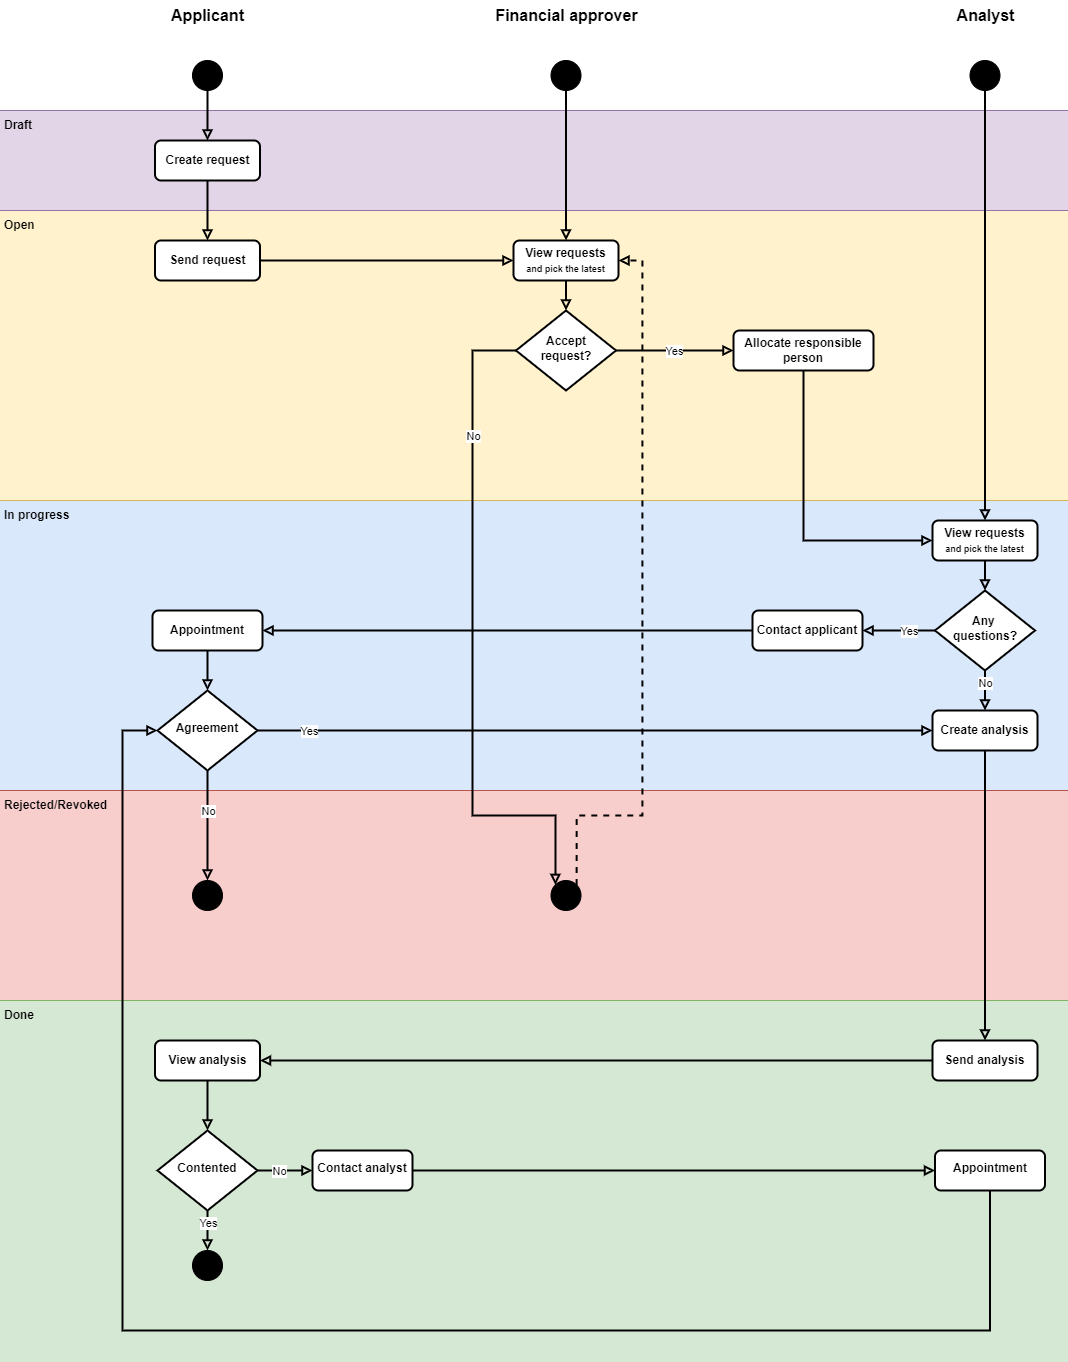
\includegraphics[scale=.4]{media/Workflow}
    \caption{Workflow}
    \label{fig:Workflow}
\end{figure}
\newpage
\section{Architektur}
Die Architektur der entwickelten Softwarelösung basiert auf modernen, skalierbaren und wartbaren Technologien, die auf die spezifischen Anforderungen des Projekts abgestimmt sind. Das System besteht aus drei Hauptkomponenten: dem Backend, das mit NestJS entwickelt wurde, dem Frontend das auf React basiert und einer relationalen Datenbank, die durch PostgreSQL unterstützt wird. Um eine flexible und isolierte Datenbankumgebung zu gewährleisten wird PostgreSQL über Docker containerisiert, was eine einfache Bereitstellung und Verwaltung verschiedener Entwicklungs- und Produktionsumgebungen ermöglicht (s. Abbildung \ref{fig:Architekturdiagramm}). 
\newline
\newline
Das Frontend wird im Rahmen einer Microfrontend-Architektur entwickelt, bei der das React-basierte Interface als eine von mehreren Anwendungen innerhalb eines größeren Systems integriert wird. Diese Architektur ermöglicht es, unterschiedliche Frontends, die mit verschiedenen Technologien entwickelt wurden, nahtlos zu kombinieren und gleichzeitig eine modulare Struktur beizubehalten. Jede Anwendung (Microfrontend) ist in sich eigenständig, kann aber über standardisierte Schnittstellen miteinander kommunizieren. Auf diese Weise können unterschiedliche Technologien und Teams gleichzeitig an verschiedenen Microfrontends arbeiten, was die Flexibilität und Skalierbarkeit des Systems erhöht.
\newline
\newline
NestJS bietet eine robuste und strukturierte Grundlage für die Backend-Entwicklung. Die serviceorientierte Architektur in Kombination mit der \ac{MVC}-Ansatz, wie ihn NestJS vorgibt, stellt sicher, dass die Geschäftslogik effizient isoliert und die verschiedenen Komponenten voneinander getrennt sind.
\newline
Die Kommunikation zwischen den einzelnen Komponenten erfolgt über klar definierte Schnittstellen und standardisierte Protokolle. Das Frontend interagiert mit dem Backend über HTTP-APIs unter Verwendung von RESTful-Endpunkten. Diese APIs ermöglichen eine effiziente und flexible Kommunikation zwischen Benutzeroberfläche und Serverlogik, wobei JSON als Standardformat für die Datenübertragung verwendet wird.
\newline
Das NestJS-Backend übernimmt die zentrale Rolle in der Geschäftslogik des Systems. Es stellt den Datenzugriff auf die PostgreSQL-Datenbank bereit und kümmert sich um die Verarbeitung der Daten. Die Datenbank wird über ein \ac{ORM} angesprochen, in diesem Fall ein TypeORM, was eine effiziente und strukturierte Kommunikation zwischen den Anwendungen und der relationalen Datenbank ermöglicht. Zusätzlich gibt es die Schnittstelle zum IAV Merida Hub, die den Import von Flotten und Fahrzeugdaten in die lokale Datenbank ermöglicht. Durch die asynchrone Kommunikation über API-Aufrufe bleibt die Datenbasis stets aktuell und wird in Echtzeit mit dem IAV Merida Hub synchronisiert.
Mittels der folgenden Abbildung wird verdeutlicht, wie die einzelnen Schichten miteinander kommunizieren.
\begin{figure}[H]
    \centering
    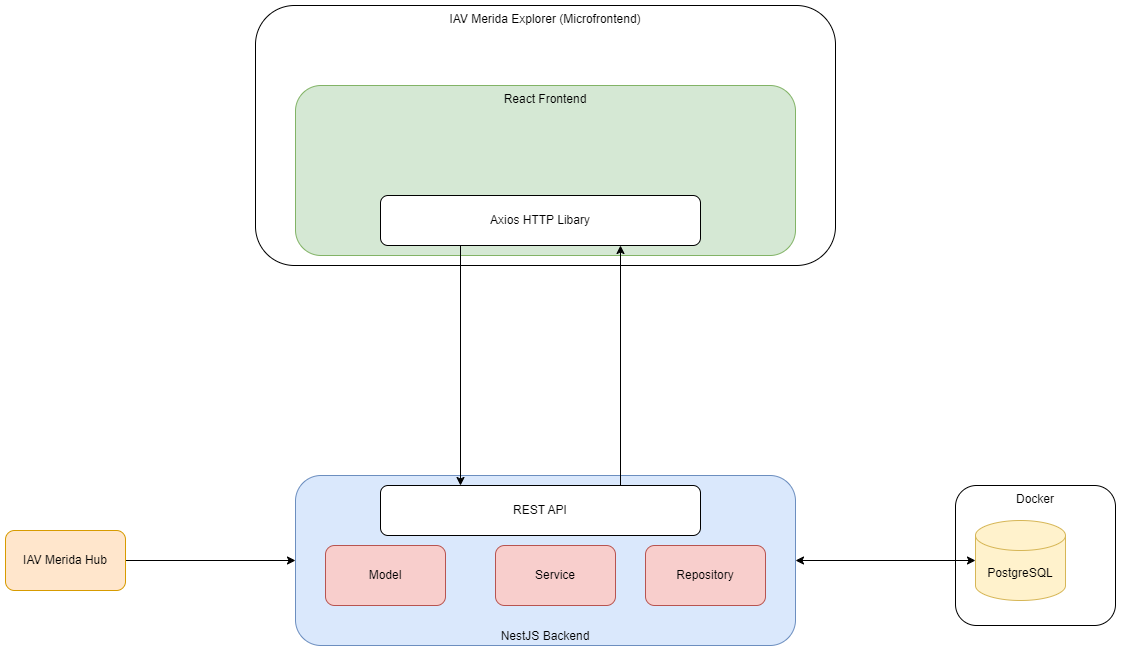
\includegraphics[scale=.4]{media/Architekturdiagramm}
    \caption{Architekturdiagramm}
    \label{fig:Architekturdiagramm}
\end{figure}
Ein zusätzliches Komponentendiagramm (s. Abbildung \ref{fig:Komponentendiagramm}) zeigt die Schnittstellen zwischen Backend, Frontend und Datenbank sowie die Verbindung zu externen Systemen. Es verdeutlicht, wie das Backend die im IAV Merida Hub gespeicherten Flotten- und Fahrzeugdaten abruft, sodass Nutzer im Frontend Flotten und – optional – Fahrzeuge auswählen kann, für die sie Messdaten und Analysen einsehen möchten.
\newline
Neben dem Merida Request-Modul bietet der IAV Merida Explorer aktuell weitere Module. Dazu gehören der Merida Transmitter für den gesicherten und automatisierten Upload von Messdaten aus verschiedenen Quellen, der Merida Signals Web für einen direkten Einblick in die verfügbaren Messdaten sowie der Merida Finder, der durch eine spezielle Suchmaske komplexe Suchanfragen über alle Messungen hinweg ermöglicht. Das Merida Dashboard visualisiert schließlich verschiedene Analysen der gesammelten Daten.
\newline
Für die Zukunft ist die Integration einer Schnittstelle zu Confluence geplant, um den Analysten eine erleichterte Dokumentation einzelner Anfragen zu ermöglichen.
\newline
Außerdem ist noch unklar, wie die Verwaltung der Daten- und Analyseanfragen erfolgen soll. Im Gespräch ist derzeit Jira, das als Ticketsystem für Anfragen dienen könnte, um die Zuweisung an Analysten zu erleichtern und einen besseren Überblick über die offenen Aufgaben zu gewährleisten. Allerdings gab es in der Vergangenheit einige Schwierigkeiten mit Jira, weshalb noch zu prüfen ist, ob Jira tatsächlich eine geeignete Lösung darstellt oder ob eine Eigenimplementierung sinnvoller wäre.
\begin{figure}[H]
    \centering
    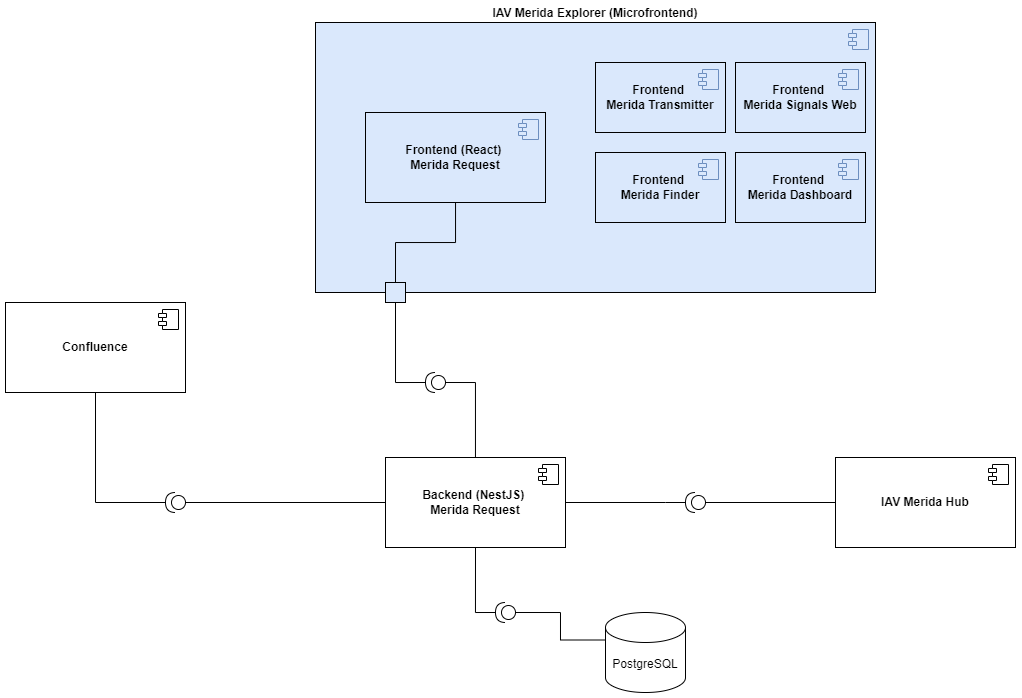
\includegraphics[scale=.4]{media/Komponentendiagramm}
    \caption{Komponentendiagramm}
    \label{fig:Komponentendiagramm}
\end{figure}
\label{chap:kapitel5}